\documentclass[tikz]{standalone}

\begin{document}

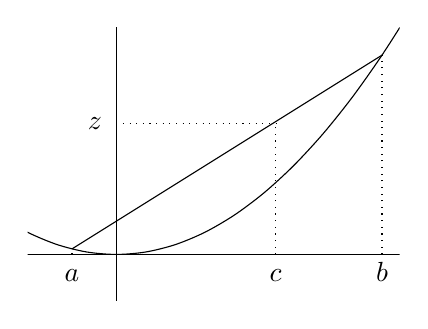
\begin{tikzpicture}[scale=4.5]
\clip (-0.25, -0.13) rectangle (0.8,{ 0.8*0.8 });
\usetikzlibrary{calc}
  \draw (-1, 0) -- (1, 0);
  \draw (0, -0.25) -- (0, 1);
  \draw[domain=-1:1, smooth] 
    plot ({\x}, {\x * \x});
  % \draw[fill=black]
  %   (0.25, {0.25 * 0.25})
  %   circle (0.025);
  \draw (-0.125, {0.125 * 0.125}) -- (0.75, {0.75 * 0.75});
  % \draw[fill=black] (0.75, {0.75 * 0.75}) circle (0.025);
  \node at (-0.125, -0.06) {$a$};
  \node at (0.75, -0.05) {$b$};
  \node at (0.45, -0.06) {$c$};
  \draw[dotted] (0.45, 0) -- (0.45, 0.37);
  \draw[dotted] (0, 0.37) -- (0.45, 0.37);
  \draw[dotted] (-0.125, 0) -- (-0.125, {0.125*0.125});
  \draw[dotted] (0.75, 0) -- (0.75, {0.75*0.75});
  \node at (-0.06, 0.37) {$z$};
\end{tikzpicture}
\end{document}
